\documentclass[9pt,twocolumn,twoside,]{pnas-new}

%% Some pieces required from the pandoc template
\providecommand{\tightlist}{%
  \setlength{\itemsep}{0pt}\setlength{\parskip}{0pt}}

% Use the lineno option to display guide line numbers if required.
% Note that the use of elements such as single-column equations
% may affect the guide line number alignment.


\usepackage[T1]{fontenc}
\usepackage[utf8]{inputenc}

% Pandoc citation processing
\newlength{\csllabelwidth}
\setlength{\csllabelwidth}{3em}
\newlength{\cslhangindent}
\setlength{\cslhangindent}{1.5em}
% for Pandoc 2.8 to 2.10.1
\newenvironment{cslreferences}%
  {}%
  {\par}
% For Pandoc 2.11+
\newenvironment{CSLReferences}[3] % #1 hanging-ident, #2 entry sp
 {% don't indent paragraphs
  \setlength{\parindent}{0pt}
  % turn on hanging indent if param 1 is 1
  \ifodd #1 \everypar{\setlength{\hangindent}{\cslhangindent}}\ignorespaces\fi
  % set line spacing
  % set entry spacing
  \ifnum #2 > 0
  \setlength{\parskip}{#3\baselineskip}
  \fi
 }%
 {}
\usepackage{calc} % for \widthof, \maxof
\newcommand{\CSLBlock}[1]{#1\hfill\break}
\newcommand{\CSLLeftMargin}[1]{\parbox[t]{\maxof{\widthof{#1}}{\csllabelwidth}}{#1}}
\newcommand{\CSLRightInline}[1]{\parbox[t]{\linewidth}{#1}}
\newcommand{\CSLIndent}[1]{\hspace{\cslhangindent}#1}


\templatetype{pnasresearcharticle}  % Choose template

\title{Demographically Stuck by Climate Change: Sea-Level Rise Migration
in the United States.}

\author[a,1,2]{Mathew E. Hauer}
\author[a,b]{Sunshine Jacobs}
\author[c]{Scott A. Kulp}

  \affil[a]{Department of Sociology, Florida State University}
  \affil[b]{Center for Demography and Population Health, Florida State
University}
  \affil[c]{Climate Central}


% Please give the surname of the lead author for the running footer
\leadauthor{Anonymous}

% Please add here a significance statement to explain the relevance of your work
\significancestatement{Authors must submit a 120-word maximum statement
about the significance of their research paper written at a level
understandable to an undergraduate educated scientist outside their
field of speciality. The primary goal of the Significance Statement is
to explain the relevance of the work in broad context to a broad
readership. The Significance Statement appears in the paper itself and
is required for all research papers.}


\authorcontributions{Please provide details of author contributions
here.}

\authordeclaration{The authors declare no conflict of interest.}

\equalauthors{\textsuperscript{1} A.O.(Author One) and A.T. (Author Two)
contributed equally to this work (remove if not applicable).}

\correspondingauthor{\textsuperscript{2} To whom correspondence should
be addressed. E-mail:
\href{mailto:mehauer@fsu.edu}{\nolinkurl{mehauer@fsu.edu}}}

% Keywords are not mandatory, but authors are strongly encouraged to provide them. If provided, please include two to five keywords, separated by the pipe symbol, e.g:
 \keywords{  one |  two |  optional |  optional |  optional  } 

\begin{abstract}
The warnings of sea-level rise driven migration first appeared in the
scientific literature in the late 1970s when increased recognition that
disintegrating ice sheets could drive people to migrate from coastal
cities. Here, we combine demographic models, flood hazard models, and a
machine learning model built on 40 years of environmental migration in
the US to project the US population distribution of US counties,
accounting for anticipated demographic change, migration probabilities,
and sea-level rise. We find that population momentum results suggest
that the demographic implications of climate migration go far beyond
simple displacement estimates, as population momentum from climate
migrants multiplies the demographic effects in both origin and
destination areas.
\end{abstract}

\dates{This manuscript was compiled on \today}
\doi{\url{www.pnas.org/cgi/doi/10.1073/pnas.XXXXXXXXXX}}

\begin{document}

% Optional adjustment to line up main text (after abstract) of first page with line numbers, when using both lineno and twocolumn options.
% You should only change this length when you've finalised the article contents.
\verticaladjustment{-2pt}

\maketitle
\thispagestyle{firststyle}
\ifthenelse{\boolean{shortarticle}}{\ifthenelse{\boolean{singlecolumn}}{\abscontentformatted}{\abscontent}}{}

% If your first paragraph (i.e. with the \dropcap) contains a list environment (quote, quotation, theorem, definition, enumerate, itemize...), the line after the list may have some extra indentation. If this is the case, add \parshape=0 to the end of the list environment.

\acknow{Please include your acknowledgments here, set in a single
paragraph. Please do not include any acknowledgments in the Supporting
Information, or anywhere else in the manuscript.}

Scientists first sounded the alarm of potential ``major dislocations in
coastal cities'' (1) due to a disintegrating West Antarctic Ice Sheet
and sea-level rise more than forty years ago. Since those early
warnings, experts continue to regard sea-level rise as one of the most
costly and visible future impacts of global climate (2--4). With the
global coastal population projected to eclipse one billion people this
century (5), sea-level rise is expected to affect and, in many cases,
displace hundreds of millions of people (3, 6).

While the scientific community understands that climate change and
sea-level rise will affect millions of people in the United States and
across the world, we face a critical knowledge gap about the impacts of
rising sea levels on human migration. Previous attempts to model
sea-level rise and migration eschew two key considerations.

First, scientists have chosen to model migrants as age-less and sex-less
individuals (6--9), ignoring the well-established relationship between
migration propensity and demographic characteristics (10--12). In
particular, the near universal age schedule of migration, with older
populations the least likely age groups to migrate and young adults the
most (\textbf{Figure 1}), suggests SLR migration is most likely to occur
among working-age adults. The age schedule of migration in conjunction
with the anticipated global, demographic shift toward a considerably
older population at the end of the century (13), suggests the potential
emergence of ``demographically stuck'' people. By ignoring these
well-established demographic relationships, the extent to which highly
vulnerable coastal communities could experience accelerated population
aging as more youthful populations migrate away remains unknown.

Second, sea-level rise migration models lack the crucial feedback loop
whereby sea-level rise migrants alter the demographic trajectory in both
their origin and destination. If sea-level rise forces millions of
people further inland, a potential domino effect could result, further
enhancing population growth in more distant locations and further
suppressing population growth to coastal areas (14--16). {[}WHAT DOES
THIS CAUSE US TO MISS?{]}

\begin{figure}
\centering
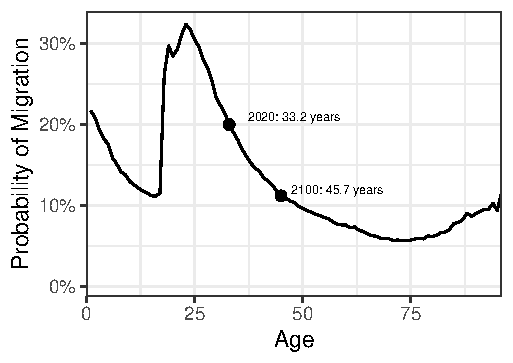
\includegraphics{FigProbMig.pdf}
\caption{Probability of Migrating by Age and Median Age in 2020 and 2100
in the United States. Figure generated using IPUMS-USA data (17). Median
age is calculated based on Shared Socioeconomic Pathway 2 (18). Barring
any additional information, this curve suggests that migration will
lessen as the US population ages this century.}
\end{figure}

In this paper, we combine matrix population models, flood hazard models,
and a migration model built on 40 years of environmental migration to
project the United States' population distribution, accounting for
anticipated demographic change, migration probabilities, and sea-level
rise. This approach allows us to investigate the potential for
accelerated aging in coastal communities and the potential for
``demographically trapped'' peoples and the temporal and demographic
dimensions of anticipated sea-level rise migration.

To investigate SLR migration, we produce three separate population
populations using a multi-regional Leslie matrix that takes the
following general form

\[
\mathbf{P_{t+1}} = \underbrace{\underbrace{\mathbf{M_t}(\mathbf{\hat{S_t}}\mathbf{P_t} - \overbrace{\mathbf{S_t}\mathbf{P_t}}^{Base})}_{Inundation} + \mathbf{\hat{S_t}}\mathbf{P_t}}_{Migration}
\tag{1}
\]

Where \(\mathbf{P_{t+1}}\) is the population at time \(t+1\),
\(\mathbf{S_{t}}\) is a Leslie matrix containing the age-sex specific
probabilities of fertility and survival, \(\mathbf{\hat{S}}_t\) is a
Leslie matrix populated with the results of a displacement model, and
\(\mathbf{M}_t\) is a matrix containing the probability of migrating
from county \(i\) to county \(j\).

We derive three population projections. \(\mathbf{S_tP_t}\) is our
\texttt{Base} population projection and represents a projection agnostic
to climate change. \(\mathbf{\hat{S_t}P_t} - \mathbf{S_tP_t}\) is our
\texttt{Inundation} projection, representing a similar projection to
those undertaken in the broader literature (e.g. (7, 9, 19). Our full
model, which we refer to as \texttt{Migration}, accounts for population
dynamics in origins and destinations.

We populate our matrices from multiple data sources. \(\mathbf{P_t}\)
come from the National Vital Statistics System (NVSS) U.S. Census
Populations with Bridged Race Categories Dataset. \(\mathbf{M_t}\)
contains the probability of migrating from each county to each county
based on the IRS county-to-county migration data. The annual series of
county-to-county migration data cover 95 to 98 percent of the tax-filing
universe (or approximately 87\% of US households (20)) and their
dependents making these data the largest migration data source for count
flows between counties in the United States. Finally, \(\mathbf{S_t}\)
and \(\mathbf{\hat{St}}\) are populated with cohort-change ratios (CCRs)
from the NVSS population data.

\(\mathbf{\hat{S_t}}\) contains the same information as \(\mathbf{S_t}\)
but reduced based on the percentage of population we anticipate will be
displaced by SLR. We arrive at this reduction with a simple,
parsimonious model fit with US counties between 1980 and 2018 with
SHELDUS verified large (\textgreater4\(\sigma\)) population declines
(n=48 such county-years). We estimate exposure to SLR as a percentage of
the population in each county using a bathtub model of inundation based
on the population-weighted area under the 95th percentile of RCP4.5 (for
a 2100 SLR amount of \textasciitilde0.9M). All population results are
reported based on SSP2.

Finally, \(\mathbf{M_t}\), \(\mathbf{S_t}\), and \(\mathbf{\hat{S_t}}\)
are projected forward using ARIMA(0,1,1) (\(\mathbf{S_t}\) and
\(\mathbf{\hat{S_t}}\)) and ETS models (\(\mathbf{M_t}\)) to capture
potential changes in demographic rates.

\hypertarget{results}{%
\section*{Results}\label{results}}
\addcontentsline{toc}{section}{Results}

We find that 0.9m of SLR compromises the land area home to 3.4 million
people between 2020 and 2100. In this simple model, the demographic
impact of SLR is 3.4 million people migrating to other places for a net
demographic change of just 3.4 million people. However, when one
accounts for population dynamics, the actual \emph{demographic} impact
of 3.4 million migrants is 12.96 million people. This is due to the
population momentum we expect to occur due to the interacting effects of
basic demographic component processes of migration, fertility, and
mortality. Most surprising is that this demographic effect is
considerably more pronounced than the simple displacement effect -- in
fact, it is nearly four times larger!

\begin{figure*}
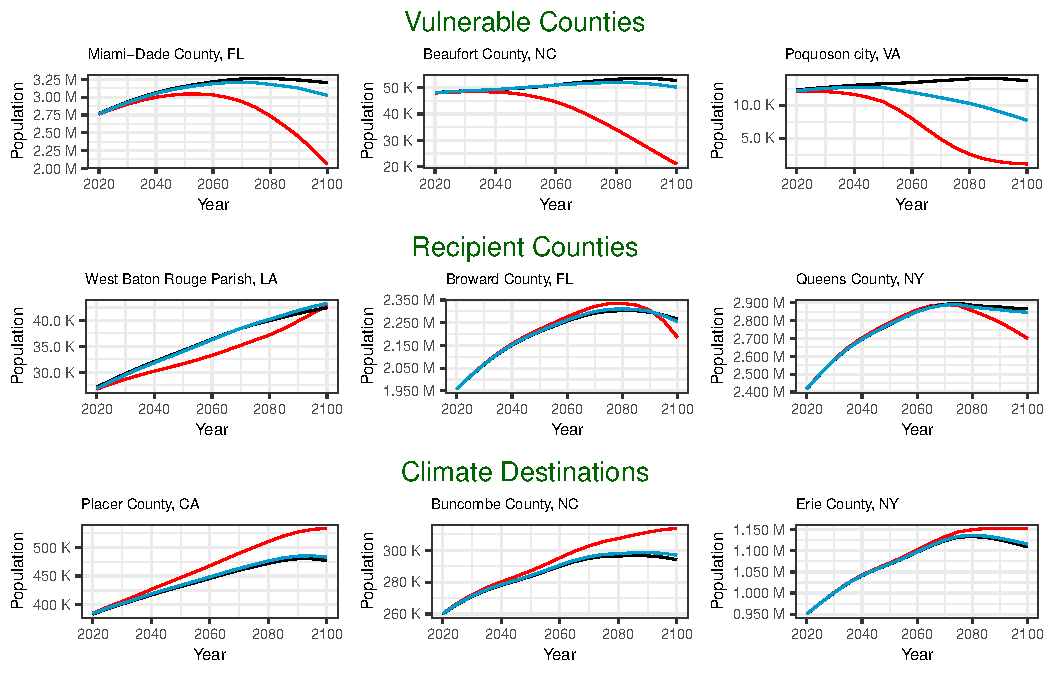
\includegraphics{FigProjLines.pdf}\label{FigProjLines}
\caption{\textbf{A comparison of base, inundation, and migration projections for four sample counties over the next century with 3ft of SLR.} We adopt the general climate migration typology as proposed by \citep{marandi2021vulnerable}. The inundation model projection refines the previous base model as it accounts for sea-level rise displacement. Including demographic processes further sophisticates the migration projection. In the case of these example counties, the migration model reflects both those who emigrated and their lost progeny, indicating a substantial decline in the projected population for 2100 as compared to the base model population.}
\end{figure*}

Furthermore, \textbf{Figure 2} shows this population momentum effect for
example nine counties following the general typology of climate
migration put forth by (16). Here, the three counties in the `Vulnerable
Counties' (those most exposed to a climate hazard) all experience
considerably pronounced demographic declines, even with rather marginal
displacements. In the case of Miami-Dade, 0.9m of SLR suggests 251K
migrants by 2100 but a total demographic impact of 1.4M people. The same
larger total demographic impact compared to simple displacement is also
present in Beaufort () and Poquoson ().

In the `Climate Destinations' (counties considered `climate havens'), we
see a similar, though reversed, pattern of population trajectories to
`Vulnerable Counties.' Here, Place CA (home to Lake Tahoe), Buncombe NC
(home to Asheville), and Erie NY (home to Buffalo), all exhibit
considerably larger demographic impacts when accounting for population
dynamics compared to just a simple displacement model. In the case of
Erie NY, this finding echoes many suggestions that Buffalo might become
a climate haven this century {[}CITES{]}.

In the `Recipient Counties' (counties closest to heavily threatened
counties), we see three separate population trajectories and
demonstrates the non-linearity in population change. West Baton Rouge,
threatened by SLR early this century, appears to be a Vulnerable County
until the middle of the century, where population momentum carries it
below an anticipated projection without SLR. Yet by the tail end of the
century, West Baton Rouge's population momentum carries it above even a
climate agnostic projection, suggesting it transitions into a Climate
Destination. Given the extreme precarity of coastal Louisiana, West
Baton Rouge and similar nearby Louisiana Parishes could transition from
Vulnerable to Climate Destination.

This is in stark contrast to Broward FL, immediately north of
Miami-Dade, and Queens NY. Here, both counties appear as climate
destinations in the early part of the century. But SLR also threatens
Broward and Queens and demographic change turns sharply negative in the
latter part of this century. Unlike West Baton Rouge, these counties
could initially be a Climate Destination only to turn into a Vulnerable
County as the century progresses. These results suggest that many people
and their descendants could find themselves exposed and displaced by SLR
as presently safe areas become increasingly vulnerable over time.

\begin{figure}
\centering
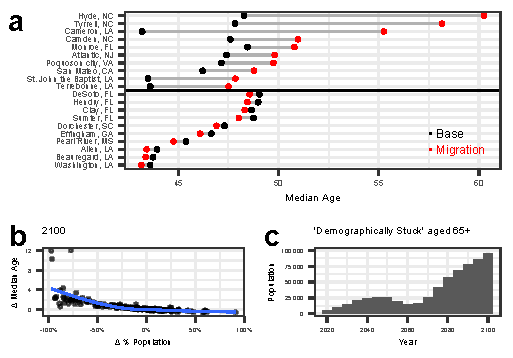
\includegraphics{FigAging.pdf}
\caption{Population Aging and `Demographically Stuck' populations. (a)
shows the ten counties with the most and least aging due to SLR
migration. (b) shows the relationship between population decline due to
SLR and aging by 2100. (c) shows an example of a county with
demographically stuck people.}
\end{figure}

\textbf{Figure 3} shows the impact of population processes on aging
related to climate migration. We find that as the percentage of the
population lost due to climate migration-related population processes
increases, the median age in the population also increases
(\textbf{Figure 3a}). Conversely, counties receiving the greatest
increase actually exhibit more \emph{youthful} populations. This effect
is particularly pronounced in some counties where the increase in median
age can approach +12 years in some highly impacted coastal counties due
to SLR migration.

We also find an example of how these three processes -- population
aging, reduced propensity to migrate among older populations, and SLR
migration -- combine to potentially create `demographically stuck'
populations. \textbf{Figure 3b} shows one such county, Cameron Parish
LA. Here, a climate agnostic population projection shows the county
slowly gaining population this century and a simple inundation model
shows the county steadily losing population. However, the fully
integrated population model suggests a striking, non-linear potential
population pathway. The parish rapidly loses population until the middle
of the century, before slowly increasing in population, eventually
yielding a larger population in 2100 compared to the simple inundation
model. We believe this is emblematic of the potential for emerging,
`demographically stuck' populations that more simplistic displacement
models will miss.

\begin{figure*}
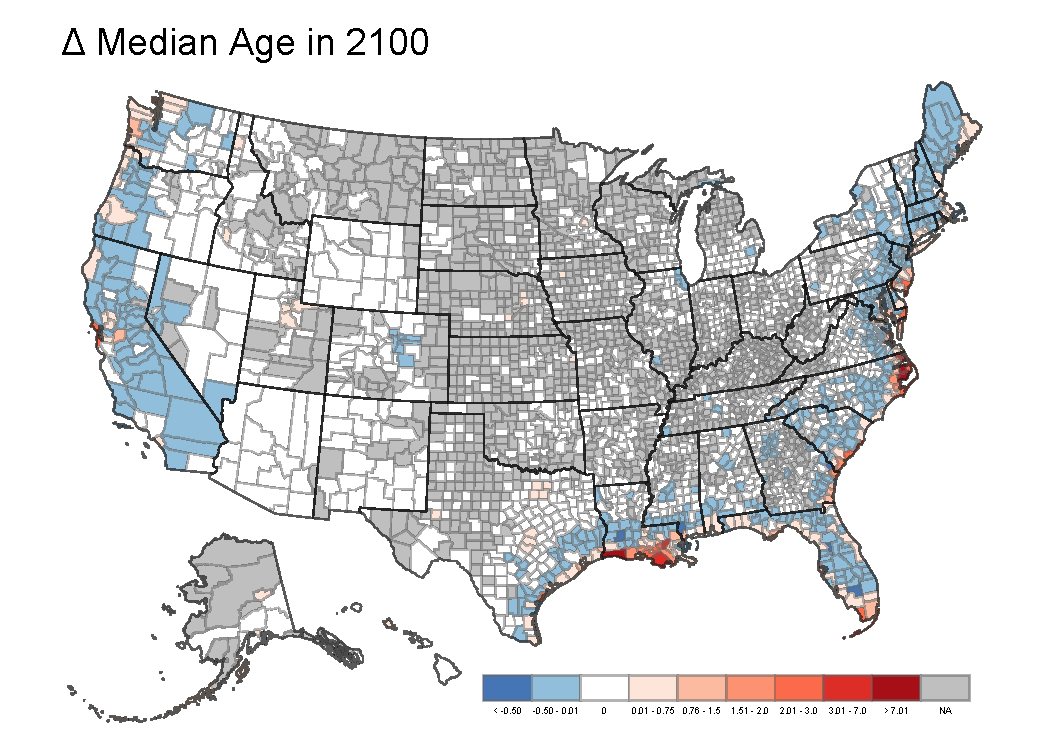
\includegraphics{FigMedAgeMap.pdf}\label{FigMedAgeMap}
\caption{\textbf{A comparison of base, inundation, and migration projections for four sample counties over the next century with 3ft of SLR.} Additional caption.}
\end{figure*}

\textbf{Figure 4} shows this increased aging across space and reveals
several important patterns. First, most coastal counties see increased
population aging by 2100 and most coastal-adjacent counties will
experience a more youthful population compared to a demographically
agnostic projection. Most migration operates within kin and social
networks within relatively short-distances and across pre-existing
migration pathways (21). Second, SLR impacts are hyperlocalized with the
majority of heavy population aging limited to select areas in Louisiana,
the Outer Banks of North Carolina, and the San Francisco Bay Area. And
Third, additional non-linearity emerges as some coastal counties can
experience reverse aging and some inland counties can experience aging
due to climate migration.

\hypertarget{discussion}{%
\section*{Discussion}\label{discussion}}
\addcontentsline{toc}{section}{Discussion}

We Discuss that

\hypertarget{conclusion}{%
\section*{Conclusion}\label{conclusion}}
\addcontentsline{toc}{section}{Conclusion}

We Discuss that

\hypertarget{format}{%
\subsection*{Materials and Methods}\label{format}}
\addcontentsline{toc}{subsection}{Materials and Methods}

To answer our research questions, we employ three main modules. The
first is the development of a parsimonious, one-dimensional,
age-specific displacement model. The second is a multiregional Leslie
matrix specification. The third is a sea-level rise exposure model.

\textbf{Parimonious, one-dimensional, age-specific displacement model.}
Our displacement model makes use of a statistical time series outlier
detection technique to first identify anomalous demographic behavior in
a time series and then verify that this anomalous behavior is associated
with an environmental event.

We use a statistical time series outlier detection algorithm (22),
implemented in the R programming language (23) via the tsoutliers
package (24).

This algorithm iteratively uses ARIMA models to 1) identify potential
outliers and 2) refit the ARIMA with the outliers removed to produce a
counter-factual time series. First, an ARIMA model is fit to the time
series using the \texttt{forecast} package in R (25, 26) where the best
performing ARIMA model is selected based on the Bayesian information
criterion (BIC). Finally, the residuals from the forecast are checked
for their significance where only outliers above a critical
\emph{t}-static are considered ``true'' outliers (\(|\tau| \geq 4\);
p-value \textless{} 0.000063). We chose this threshold to minimize the
probability of committing a Type I error (or claiming an outlier is true
when it is, in fact, not).

We use this outlier detection algorithm to search over county population
totals for the time period 1980-2018. We use the National Vital
Statistics System (NVSS) U.S. Census Populations with Bridged Race
Categories data set. The NVSS Bridged Race Categories data set
harmonizes racial classifications across disparate time periods to allow
population estimates to be sufficiently comparable across space and
time. Importantly, all county boundaries are rectified to be
geographically consistent across all time periods. We use the the
1969-2018 dataset, but the historical population estimates prior to 1980
display unusual volatility, so we consider only the time periods
1980-2018. We also only consider counties created prior to year 2000 and
contained in the NVSS data.

We search all US counties for negative statistical outliers (indicating
population losses) between 1980 and 2018. We detect 52 county-years with
population losses of magnitude 4\(\sigma\) or greater (see
\textbf{Supplementary Table X} for the details of these county-years).
We then use the Spatial Hazard Events and Losses Database for the United
States (SHELDUS) (27), a county-level hazard data set for the US which
contains information about the direct losses (property and crop losses,
injuries, and fatalities) caused by a hazard event (thuderstorms,
hurricanes, floods, wildfires, tornados, flash floods, earthquakes,
etc.) for the period 1960 to the present. We use SHELDUS to ensure the
county time periods we identify as statistical outliers with population
losses experienced an environmental hazard in that county-year with per
capita hazardous losses in excess of the 50th percentile. This is to
ensure the outlier population losses that we detect are associated with
a hazard rather than other forces, such as economic forces.

Four county-periods either were not in the SHELDUS database or
experienced per capita hazard losses below the 50th percentile.
Additionally, one county-period contained age-sex groups with 0 people,
necessitating exclusion. The remaining 48 environmental events include
tornados, wind damage, winter weather, earthquakes, flooding, tropical
cyclones, hail, and other environmental hazards. Using this universe of
48 county-periods exhibiting large population declines after verified
hazard losses, across over 40 years and across a wide variety of
environmental hazards, we then build a flexible, one-dimensional,
age-specific displacement model.

To link population displacement with age-specific population changes, we
calculate cohort-change ratios (CCRs) in each county using the NVSS
population data for the period 1969-2018. Cohort-change ratios take the
following general form (see (28, 29) for a more detailed description):

\[CCR_{x,t}  =  \frac{_nP_{x,t}} {_nP_{x-y,t-y}} \tag{2}\]

Where \(_nP_{x,t}\) is the population aged \(x\) to \(x+n\) in time
\(t\) and \(_nP_{x-y,t}\) is the population aged \(x-y\) to \(x+n-y\) in
time \(t\) where \(y\) refers to the time difference between time
periods. Since mortality must decrement a population, any CCR above 1.0
implies a net-migration rate in excess of the mortality rate, and a
growing population.

We build the following model based on the relationship between the
change in CCRs at age \(x\), \(\Delta CCR_x = CCR_{x,t} / CCR_{x,t-1}\),
and the percentage decline in the total population compared to the
counter-factual in the outlier detection method,
\(\Delta P_t = \hat{P_t} / P_t\):

\[log(\Delta CCR_x) = a_x + b_xh \tag{3}\]

Here, \(h\) is the log(\(\Delta P_t\)) and shows a linear relationship
with the logarithm of the change in CCRs by age. \(x\) refers to
five-year age groups: 0-4, 5-9,\ldots, 85+. This is a similar model and
approach to Wilmoth et al.'s (30) flexible, one-dimensional mortality
model based on the linearity between age-specific mortality rates and
infant mortality. \textbf{Supplementary Table 1} depicts the correlation
coefficients between log(\(\Delta CCR_x\)) and log(\(\Delta P_t\)). The
age groups with the lowest correlation coefficients are young adult
males aged 20-39 and those in the open-ended age interval (80+),
suggesting these age/sex groups react to environmental signals the least
predictably.

Using \(h=log(\Delta P_t)\), we can estimate age-specific changes in
CCRs after an environmental event by simply applying the following
formula:

\[\hat{CCR_{x,t}} = CCR_{x,t-1} \cdot e^{\hat\beta_xh} \tag{4}\]

Where \(e^{\hat\beta_xh}\) provides the percentage change in \(CCR_x\)
based on the log(\(\Delta{P_t}\)).In this case, we drop the intercept
(\(a\)) from the estimation procedure to ensure a 0\% decline in
population yields a corresponding 0\% change in the CCR. Multiplying the
result from the model with the CCR in the year prior yields the
anticipated change in the CCR. These changes in CCRs can then be applied
to any time series of population values to generate an anticipated
population.

We estimate the predicted population using the equation outlined above
and then compare it against the observed population.
\textbf{Supplementary Figure 1} shows the accuracy of our fitted,
one-dimensional model. Regarding the total population in our 48
counties, our model performs well with an \(r^2\) value of 0.994 and
performs well regardless of population size. Regarding each individual
\(P_x\) group, our model still performs quite well with an \(r^2\) of
0.976. Just like with the total population, the accuracy of our model
does not depend on population size.

\textbf{Sea-level Rise Exposure}. To estimate the populations at-risk to
SLR and thus the value \(h\) in \emph{Equation 4}, we employ inundation
modeling (15) which assumes that people who are underwater 100\% of the
time must migrate. We estimate these populations using airborne
lidar-derived digital elevation models (DEMs) produced by NOAA and
supplemented with both the USGS Northern Gulf of Mexico Topobathymetric
DEM in Louisiana and the USGS National Elevation Dataset in the fraction
of land not covered by other sources (see (31) for details on the
construction of the DEMs).

Using a bathtub model of inundation, we calculate the land area under a
given water height to generate binary inundation surfaces. SLR exposure
is hyperlocalized, and we generate this inundation area in the Census
Block Groups (CBG; n=81,815) located in coastal counties (n=406)
expected to experience any probability of flooding. We use probabilistic
SLR projections (32, 33) that are closely aligned with the IPCC for our
water heights. To calculate the land area under a given water height, we
simply threshold the DEM to find pixels below \(SLR_{yt}\) where \(y\)
is the projected height of SLR in a given year \(t\). For each CBG, we
simply calculate the percentage of its pixels on dry land (defined in
the National Wetland Inventory (34)) covered by the inundation surface
and multiply this percentage by the total population in the CBG in year
\(t\) to produce the total number of people at-risk to a given amount of
SLR in a given year. We then aggregate these CBGs to the county-level to
calculate the percentage of people in a given county at-risk of
inundation.

To account for potential sub-county shifts in population, we use a
sub-county demographic projection to produce spatiotemporally consistent
CBG boundaries for the period 1940-2010 and project these populations
forward using a mixed, linear/exponential projection for the period
2010-2100. We use the `Year Structure Built' question from the 2013-2018
US Census Bureau's ACS to calculate the number of housing units \(H\) in
each CBG. We calculate \(H\) in th eperiod 1940-2010 using
\(\hat{H}^v_{ij} = \left( \frac{C^v_j}{\sum_{i=1}^{n}\sum_{t=1939}^{v-1} H^v_{ijt}} \right) \cdot \displaystyle\sum_{t=1939}^{v-1} H_{ijt}^{v}\),
where \(C_j^v\) is the number of HUs in county \(j\) counted in census
taken in time \(v\), \(H^v_{ij}\) is the number of HUs in block group
\(i\) in county \(j\) based on the ``year structure built'' question in
the ACS, and \(v\) is the set of time periods
\(v\in\{1940,1950,1960,1970,1980,1990,2000,2010\}\). We then project
these housing unit values using a linear projection for any CBG
experiencing population growth and an exponential projection for any CBG
experiencing population decline. See (35, 36) for more details.

We convert \(H\) to population \(P\) via the Housing Unit Method of
population estimation (\(P_t = H \cdot PPHU\)) where the population is
given as the number of people per housing unit (\(PPHU\)) multiplied by
the number of housing units (\(H\)). Using a similar approach as
estimating \(H\), we estimate the population in each time period with
\(P^{'v}_{ij} = \frac{P^v_j}{\sum \Big[ \Big( \frac{PPHU_{ij}^{2018}}{PPHU_j^{2018}} \cdot PPHU_j^v \Big) \cdot \hat{H}^v_{ij} \Big]} \cdot \hat{P}^v_{ij}\)
where the \(PPHU\) in 2018 from the ACS is denoted as
\(PPHU^{2018}_{ij}\) while the \(PPHU\) observed in in historical time
\(v\) from historical census data is denoted as \(PPHU_j^v\).

To calculate the percentage of the population at-risk in each county, we
multiply the percentage of each CBG inundated under a given water height
\(y\) in time period \(t\) by \(P^{'t}_{ij}\) to produce
\(P^{risk}_{ij}\). The ratio of the total population
(\(\sum{P^{risk}_{ij}}/P^{'t}_{j}\)) in each county in year \(t\) is
thus the percentage of the population in a given county at-risk of
inundation.

The percentage of the population at-risk to SLR in each county, in
essence, represents the \(\Delta P_t\) from our equations above where
\(\Delta P_t = \hat{P_t}/P_t\). In this case, \(\hat{P_t}/P_t\) is the
percentage of the population in any county at-risk of inundation. Such a
calculation allows us to seamlessly combine our parsimonious
displacement model with our matrix population model.

\textbf{Matrix Population Models} We employ the use of multiregional
leslie matrices in our population projections (37).

In a typical Leslie matrix,

\begin{equation}
    \mathbf{P_{t+1}} = \mathbf{S_t} \cdot \mathbf{P_t} \label{eq:lesliematrix_base} \tag{5}
\end{equation}

Where \(\mathbf{P_t}\) refers to the population matrix containing \(k\)
age groups and \(\mathbf{S_t}\) contains the age-specific fertility and
mortality rates.

Thus, to produce a population projection, the operation looks akin to

\begin{equation}
\begin{bmatrix}
    0 & F_2 & F_3 \\
    S_1 & 0 & 0 \\
    0 & S_2 & S_3
\end{bmatrix}
\cdot
\begin{bmatrix}
    P_1 \\
    P_2 \\
    P_3
\end{bmatrix}
=
\begin{bmatrix}
    0 & 0.2 & 0.2 \\
    0.62 & 0 & 0 \\
    0 & 0.35 & 0.35
\end{bmatrix}
\cdot
\begin{bmatrix}
    100 \\
    100 \\
    100
\end{bmatrix}
=
\begin{bmatrix}
    40 \\
    68 \\
    71
\end{bmatrix}\nonumber
\end{equation}

In a multi-regional projection model, we can use a ``super-matrix.''

A 2-region model would take the following general form for the
\(\mathbf{S_t}\) matrix,

\begin{equation}
 \mathbf{MS_{t+1}} =
\begin{bmatrix}
\begin{array}{c|c}

\mathbf{S_i} & \mathbf{M_{j\rightarrow i}} \\
\hline
\mathbf{M_{i\rightarrow j}} & \mathbf{S_j} \\

\end{array}
\end{bmatrix}\nonumber
\end{equation}

Such that the diagonal \(\mathbf{S}\) matrices contain combined
survival, fertility, and migration probabilities while the off-diagonal
\(\mathbf{M}\) matrices contain the probabilities of each age-group
moving from one region to the other.

We populate our Leslie matrices with the 3,143 US counties, 18 five-year
age groups, and two sex groups. We use CCRs to populate our \(S\) values
in each matrix and child-woman ratios to populate our \(F\) values. The
values come from the NVSS Bridged Race Categories. To project the CCRs,
We employ an autoregressive integrated moving average (ARIMA) model for
forecasting equally spaced univariate time series data. We use an
\texttt{ARIMA(0,1,1)} model, which produces forecasts equivalent to
simple exponential smoothing. All projections were undertaken in
\textbf{R} (23) using the \texttt{forecast} package (25).

We use the NVSS data for the period 1969-2018 for county \(c\), age
group \(x\), sex \(s\) in an \texttt{ARIMA(0,1,1)} to create
\(CCR_{cxst}\) for time periods \(t+1\). The initial \(\mathbf{P_1}\)
and \(\mathbf{S_t}\) matrices use the 2018 NVSS data. \(CCR_{cxst}\) is
reduced using equation (4) where \(h\) is the percentage of the
population at-risk to SLR in order to populate the
\(\mathbf{\hat{S_t}}\) matrix.

We also calculate the probability of migrating from each county to each
county and use this to populate the \(\mathbf{M_t}\) matrix. These data
come from the IRS county-to-county migration files from 1990-2018 (see
(38) and (39) for descriptions of this data). The IRS began using tax
data to estimate migration in the 1970s and 1980s (40, 41) and began
releasing migration data in 1990. The IRS uses individual federal tax
returns, matches these individual returns between two tax years (for
instance, tax year 2000 and tax year 2001), and identifies both migrants
and non-migrants. Beginning with the tax year 1991 (the migration year
1990), the IRS produces these data in conjunction with the US Census
Bureau using the IRS Individual Master File, which contains every Form
1040, 1040A, and 1040EZ (42). We identify migration when a current
years' tax form contains an address different from the preceding years'
return. A non-migrant is identified when there is no change in address
between two years. For the 2002 tax year, the IRS migration data
contained approximately 130 million returns (42).

The annual series of county-to-county migration data cover 95 to 98
percent of the tax-filing universe (or approximately 87\% of US
households (20)) and their dependents making these data the largest
migration data source for count flows between counties in the United
States. The IRS derives migration information from tax-filings making
those who do not file taxes most likely to be underrepresented in the
migration data (42, 43), namely undocumented populations, the poor, the
elderly, and college students (42). However, the overwhelming majority
of householders file US tax returns in the United States (20).

To capture changes in the migration system, we employ an ETS model
(Error, Trend, Seasonal), a univariate time series forecasting model
(44). We use an ETS model for migration instead of an ARIMA(0,1,1) as we
do for the CCRs because the CCRs are subject to multiplication during a
drift, whereas the migration system is not. A CCR that drifts from 1.1
\(\rightarrow\) 1.3 represents more than a 10-fold increase in a
projected population over our time horizons (1.1\^{}17 = 5x, 1.3\^{}17 =
86x). Projecting the migration system itself is not subject to such
exponential drift.

We fit individual ETS models for each county's numeric migrants between
each origin-destination dyadic pair using the \texttt{forecast} package
in R (25). This approach allows the underlying migration system to
evolve and change over the projection horizon, allowing dyadic pairs to
wax or wane.The model converts the numeric projections to fractions of
the total projected migrants to populate the diagonal in the
\(\mathbf{M}\) matrix above where non-migrants (i.e.~those migrating
from \(i\rightarrow i\)) are included. The result is the fraction of
individuals surviving from age group \(a\) who migrate from
\(i\rightarrow j\).

The \(\mathbf{M_t}\) matrix takes the following general form

\begin{equation}
\mathbf{M_{t}} =
\begin{bmatrix}
\begin{array}{c|c}

\begin{matrix} 1 & 0 & 0 \\ 0 & 0.85 & 0 \\ 0 & 0 & 1 \end{matrix} &
\begin{matrix} 0 & 0 & 0 \\ 0 & 0 & 0 \\ 0 & 0 & 0 \end{matrix} \\
\hline
\begin{matrix} 0 & 0 & 0 \\ 0 & 0.15 & 0 \\ 0 & 0 & 0 \end{matrix} &
\begin{matrix} 1 & 0 & 0 \\ 0 & 1 & 0 \\ 0 & 0 & 1 \end{matrix} \\
\end{array}
\end{bmatrix}
\end{equation}

Where the migration rate from \(i\) to \(j\) in age group 2 is 0.15.

We control all population projections to the Shared Socioeconomic
Pathway 2: Middle of the Road (18) and we use the 95th percentile of
RCP4.5 for our inundation scenario (45). Full results for all plausible
SSP/RCP combinations are available in the \textbf{Supplementary
Material}.

\textbf{Data Availability.} The data resulting from this study are
deposited at 10.5281/zenodo.5562904 {[}CITE{]}. The underlying data that
support the findings of this study are available from Climate Central
but restrictions apply to the availability of these data, which were
used under license for the current study, and so are not publicly
available. Data are however available from the authors upon reasonable
request and with permission of Climate Central.

\textbf{Code Availability.} Code to reproduce our analysis is available
at 10.5281/zenodo.5562904 {[}CITE{]}.

\hypertarget{acknowledgements}{%
\subsection*{Acknowledgments}\label{acknowledgements}}
\addcontentsline{toc}{subsection}{Acknowledgments}

This work was supported by the State of Louisiana, the American Society
of Adaptation Professionals, the New York State Energy Research \&
Development Authority, and the Great Lakes Integrated Sciences \&
Assessment. We would like to thank T. Gill, N. Nagle, A. Moulton, S.
Bohon, and C. Schmertmann for their early feedback and assistance. Thank
you!

\showmatmethods
\showacknow
\pnasbreak

\hypertarget{refs}{}
\begin{CSLReferences}{0}{0}
\leavevmode\hypertarget{ref-mercerWestAntarcticIce1978}{}%
\CSLLeftMargin{1. }
\CSLRightInline{Mercer JH (1978) West {Antarctic} ice sheet and {CO} 2
greenhouse effect: A threat of disaster. \emph{Nature} 271(5643):321.}

\leavevmode\hypertarget{ref-mcgranahanRisingTideAssessing2007}{}%
\CSLLeftMargin{2. }
\CSLRightInline{McGranahan G, Balk D, Anderson B (2007) The rising tide:
Assessing the risks of climate change and human settlements in low
elevation coastal zones. \emph{Environment and Urbanization}
19(1):17--37.}

\leavevmode\hypertarget{ref-nichollsSeaLevelRiseIts2010}{}%
\CSLLeftMargin{3. }
\CSLRightInline{Nicholls RJ, Cazenave A (2010) Sea-{Level Rise} and {Its
Impact} on {Coastal Zones}. \emph{Science} 328(5985):1517--1520.}

\leavevmode\hypertarget{ref-straussCarbonChoicesDetermine2015}{}%
\CSLLeftMargin{4. }
\CSLRightInline{Strauss BH, Kulp S, Levermann A (2015) Carbon choices
determine {US} cities committed to futures below sea level.
\emph{Proceedings of the National Academy of Sciences}
112(44):13508--13513.}

\leavevmode\hypertarget{ref-neumannFutureCoastalPopulation2015}{}%
\CSLLeftMargin{5. }
\CSLRightInline{Neumann B, Vafeidis AT, Zimmermann J, Nicholls RJ (2015)
Future {Coastal Population Growth} and {Exposure} to {Sea}-{Level Rise}
and {Coastal Flooding} - {A Global Assessment}. \emph{PLOS ONE}
10(3):e0118571.}

\leavevmode\hypertarget{ref-hauerMigrationInducedSealevel2017}{}%
\CSLLeftMargin{6. }
\CSLRightInline{Hauer ME (2017) Migration induced by sea-level rise
could reshape the {US} population landscape. \emph{Nature Climate
Change} 7(5):321--325.}

\leavevmode\hypertarget{ref-davisUniversalModelPredicting2018}{}%
\CSLLeftMargin{7. }
\CSLRightInline{Davis KF, Battachan A, D'Odorico P, Suweis S (2018) A
universal model for predicting human migration under climate change:
Examining future sea level rise in {Bangladesh}. \emph{Environmental
Research Letters} 13.}

\leavevmode\hypertarget{ref-de_lellis_modeling_2021}{}%
\CSLLeftMargin{8. }
\CSLRightInline{De Lellis P, Ruiz Marín M, Porfiri M (2021) Modeling
{Human} {Migration} {Under} {Environmental} {Change}: {A} {Case} {Study}
of the {Effect} of {Sea} {Level} {Rise} in {Bangladesh}. \emph{Earth's
Future} 9(4).
doi:\href{https://doi.org/10.1029/2020EF001931}{10.1029/2020EF001931}.}

\leavevmode\hypertarget{ref-rigaud2018groundswell}{}%
\CSLLeftMargin{9. }
\CSLRightInline{Rigaud KK, et al. (2018) Groundswell.}

\leavevmode\hypertarget{ref-blackClimateChangeMigration2011}{}%
\CSLLeftMargin{10. }
\CSLRightInline{Black R, Bennett SRG, Thomas SM, Beddington JR (2011)
Climate change: {Migration} as adaptation. \emph{Nature} 478:447--449.}

\leavevmode\hypertarget{ref-clarkInterpretingMigrationPrism2015}{}%
\CSLLeftMargin{11. }
\CSLRightInline{Clark WA, Maas R (2015) Interpreting migration through
the prism of reasons for moves. \emph{Population, Space and Place}
21(1):54--67.}

\leavevmode\hypertarget{ref-rogers1988age}{}%
\CSLLeftMargin{12. }
\CSLRightInline{Rogers A (1988) Age patterns of elderly migration: An
international comparison. \emph{Demography} 25(3):355--370.}

\leavevmode\hypertarget{ref-gerland2014world}{}%
\CSLLeftMargin{13. }
\CSLRightInline{Gerland P, et al. (2014) World population stabilization
unlikely this century. \emph{Science} 346(6206):234--237.}

\leavevmode\hypertarget{ref-curtisUnderstandingDemographicImplications2011}{}%
\CSLLeftMargin{14. }
\CSLRightInline{Curtis KJ, Schneider A (2011) Understanding the
demographic implications of climate change: Estimates of localized
population predictions under future scenarios of sea-level rise.
\emph{Population and Environment} 33(1):28--54.}

\leavevmode\hypertarget{ref-hauer2020sea}{}%
\CSLLeftMargin{15. }
\CSLRightInline{Hauer ME, et al. (2020) Sea-level rise and human
migration. \emph{Nature Reviews Earth \& Environment} 1(1):28--39.}

\leavevmode\hypertarget{ref-marandi2021vulnerable}{}%
\CSLLeftMargin{16. }
\CSLRightInline{Marandi A, Main KL (2021) Vulnerable city, recipient
city, or climate destination? Towards a typology of domestic climate
migration impacts in US cities. \emph{Journal of environmental studies
and sciences} 11(3):465--480.}

\leavevmode\hypertarget{ref-ruggles_steven_ipums_2021}{}%
\CSLLeftMargin{17. }
\CSLRightInline{Ruggles S, et al. (2021) {IPUMS} {USA}: {Version} 11.0.
doi:\href{https://doi.org/10.18128/D010.V11.0}{10.18128/D010.V11.0}.}

\leavevmode\hypertarget{ref-samir2017human}{}%
\CSLLeftMargin{18. }
\CSLRightInline{Samir K, Lutz W (2017) The human core of the shared
socioeconomic pathways: Population scenarios by age, sex and level of
education for all countries to 2100. \emph{Global Environmental Change}
42:181--192.}

\leavevmode\hypertarget{ref-MigrationInducedSealevel}{}%
\CSLLeftMargin{19. }
\CSLRightInline{Migration induced by sea-level rise could reshape the
{US} population landscape \textbar{} {Nature Climate Change}.}

\leavevmode\hypertarget{ref-molloy2011internal}{}%
\CSLLeftMargin{20. }
\CSLRightInline{Molloy R, Smith CL, Wozniak A (2011) Internal migration
in the united states. \emph{Journal of Economic perspectives}
25(3):173--96.}

\leavevmode\hypertarget{ref-findlayMigrantDestinationsEra2011}{}%
\CSLLeftMargin{21. }
\CSLRightInline{Findlay AM (2011) Migrant destinations in an era of
environmental change. \emph{Global Environmental Change} 21:S50--S58.}

\leavevmode\hypertarget{ref-chen1993joint}{}%
\CSLLeftMargin{22. }
\CSLRightInline{Chen C, Liu L-M (1993) Joint estimation of model
parameters and outlier effects in time series. \emph{Journal of the
American Statistical Association} 88(421):284--297.}

\leavevmode\hypertarget{ref-rcore}{}%
\CSLLeftMargin{23. }
\CSLRightInline{R Core Team (2019) \emph{R: A language and environment
for statistical computing} (R Foundation for Statistical Computing,
Vienna, Austria) Available at: \url{https://www.R-project.org/}.}

\leavevmode\hypertarget{ref-tsoutliers2019}{}%
\CSLLeftMargin{24. }
\CSLRightInline{López-de-Lacalle J (2019) \emph{Tsoutliers: Detection of
outliers in time series}.}

\leavevmode\hypertarget{ref-Rforecast}{}%
\CSLLeftMargin{25. }
\CSLRightInline{Hyndman R, et al. (2019) \emph{{forecast}: Forecasting
functions for time series and linear models} Available at:
\url{http://pkg.robjhyndman.com/forecast}.}

\leavevmode\hypertarget{ref-hymdman2008}{}%
\CSLLeftMargin{26. }
\CSLRightInline{Hyndman RJ, Khandakar Y (2008) Automatic time series
forecasting: The forecast package for {R}. \emph{Journal of Statistical
Software} 26(3):1--22.}

\leavevmode\hypertarget{ref-SHELDUS}{}%
\CSLLeftMargin{27. }
\CSLRightInline{Emergency Management and Homeland Security C for (2018)
The {Spatial} {Hazard} {Events} and {Losses} {Database} for the {United}
{States}, {Version} 17.0 {[}{Online} {Database}{]}.}

\leavevmode\hypertarget{ref-hauer2019population}{}%
\CSLLeftMargin{28. }
\CSLRightInline{Hauer ME (2019) Population projections for US counties
by age, sex, and race controlled to shared socioeconomic pathway.
\emph{Scientific data} 6(1):1--15.}

\leavevmode\hypertarget{ref-swanson2010forecasting}{}%
\CSLLeftMargin{29. }
\CSLRightInline{Swanson DA, Schlottmann A, Schmidt B (2010) Forecasting
the population of census tracts by age and sex: An example of the
hamilton--perry method in action. \emph{Population Research and Policy
Review} 29(1):47--63.}

\leavevmode\hypertarget{ref-wilmoth2012flexible}{}%
\CSLLeftMargin{30. }
\CSLRightInline{Wilmoth J, Zureick S, Canudas-Romo V, Inoue M, Sawyer C
(2012) A flexible two-dimensional mortality model for use in indirect
estimation. \emph{Population studies} 66(1):1--28.}

\leavevmode\hypertarget{ref-kulp2019new}{}%
\CSLLeftMargin{31. }
\CSLRightInline{Kulp SA, Strauss BH (2019) New elevation data triple
estimates of global vulnerability to sea-level rise and coastal
flooding. \emph{Nature communications} 10(1):1--12.}

\leavevmode\hypertarget{ref-sweetGlobalRegionalSea2017}{}%
\CSLLeftMargin{32. }
\CSLRightInline{Sweet WV, et al. (2017) Global and regional sea level
rise scenarios for the {United States}.}

\leavevmode\hypertarget{ref-koppProbabilistic21st22nd2014}{}%
\CSLLeftMargin{33. }
\CSLRightInline{Kopp RE, et al. (2014) Probabilistic 21st and 22nd
century sea-level projections at a global network of tide-gauge sites.
\emph{Earth's future} 2(8):383--406.}

\leavevmode\hypertarget{ref-WetlandInventory}{}%
\CSLLeftMargin{34. }
\CSLRightInline{U.S. Fish and Wildlife Service (2012) National wetlands
inventory website. U.s. Department of the interior, fish and wildlife
service, washington, d.c. Http://www.fws.gov/wetlands/.}

\leavevmode\hypertarget{ref-MillionsProjectedBe}{}%
\CSLLeftMargin{35. }
\CSLRightInline{Millions projected to be at risk from sea-level rise in
the continental {United~States} \textbar{} {Nature Climate Change}.}

\leavevmode\hypertarget{ref-hauerNoLandwardMovement2019}{}%
\CSLLeftMargin{36. }
\CSLRightInline{Hauer ME, Hardy RD, Mishra DR, Pippin JS (2019) No
landward movement: Examining 80 years of population migration and
shoreline change in {Louisiana}. \emph{Population and Environment}.
doi:\href{https://doi.org/10.1007/s11111-019-00315-8}{10.1007/s11111-019-00315-8}.}

\leavevmode\hypertarget{ref-rogers1966multiregional}{}%
\CSLLeftMargin{37. }
\CSLRightInline{Rogers A (1966) The multiregional matrix growth operator
and the stable interregional age structure. \emph{Demography}
3(2):537--544.}

\leavevmode\hypertarget{ref-hauer2019irs}{}%
\CSLLeftMargin{38. }
\CSLRightInline{Hauer M, Byars J (2019) IRS county-to-county migration
data, 1990--2010. \emph{Demographic Research} 40:1153--1166.}

\leavevmode\hypertarget{ref-dewaard2021user}{}%
\CSLLeftMargin{39. }
\CSLRightInline{DeWaard J, et al. (2021) User beware: Concerning
findings from the post 2011--2012 US internal revenue service migration
data. \emph{Population Research and Policy Review}:1--12.}

\leavevmode\hypertarget{ref-engels1981measuring}{}%
\CSLLeftMargin{40. }
\CSLRightInline{Engels RA, Healy MK (1981) Measuring interstate
migration flows: An origin---destination network based on internal
revenue service records. \emph{Environment and Planning A}
13(11):1345--1360.}

\leavevmode\hypertarget{ref-franklin2006pandora}{}%
\CSLLeftMargin{41. }
\CSLRightInline{Franklin RS, Plane DA (2006) Pandora's box: The
potential and peril of migration data from the american community
survey. \emph{International Regional Science Review} 29(3):231--246.}

\leavevmode\hypertarget{ref-gross2005internal}{}%
\CSLLeftMargin{42. }
\CSLRightInline{Gross E (2005) Internal revenue service area-to-area
migration data: Strengths, limitations, and current trends.
\emph{Proceedings of the Section on Government Statistics}, p 2005.}

\leavevmode\hypertarget{ref-dewaard2016population}{}%
\CSLLeftMargin{43. }
\CSLRightInline{DeWaard J, Curtis KJ, Fussell E (2016) Population
recovery in new orleans after hurricane katrina: Exploring the potential
role of stage migration in migration systems. \emph{Population and
environment} 37(4):449--463.}

\leavevmode\hypertarget{ref-hyndman2008forecasting}{}%
\CSLLeftMargin{44. }
\CSLRightInline{Hyndman R, Koehler AB, Ord JK, Snyder RD (2008)
\emph{Forecasting with exponential smoothing: The state space approach}
(Springer Science \& Business Media).}

\leavevmode\hypertarget{ref-koppProbabilistic21st22nd}{}%
\CSLLeftMargin{45. }
\CSLRightInline{Kopp RE, et al. Probabilistic 21st and 22nd {Century
Sea}-{Level Projections} at a {Global Network} of {Tide}-{Gauge Sites}.
\emph{Earth's Future} 2:383--406.}

\end{CSLReferences}



% Bibliography
% \bibliography{pnas-sample}

\end{document}
